\section{Visualizations}
We have made some renderings of the systems we have studied, as can be seen in \crefrange{fig:renderings_rough_fracture01_abel}{fig:renderings_flat_fractures02}. All renderings and visualizations were made using the program Ovito\cite{stukowski2010ovito}, using the built-in open-source ``Tachyon'' rendering engine.

In the renderings in this section we have colored the silicon atoms yellow, the oxygen atoms blue, and the hydrogen atoms white. The silicon atoms have been given a radius of 1 \AA, the oxygen atoms 0.6 \AA, and the hydrogen atoms 0.3 \AA.

% ---- rough_fracture01_abel ---- %
%
\begin{figure}[!p]%
%     \centering%
    \setlength{\myfigwidth}{0.55\textwidth}%
    \setlength{\myhfillwidth}{5mm}%
    %     \setlength{\mycaptionwidth}{0.3\textwidth}%
    %
    % Use makebox to center figures below that are wider than \textwidth
    % Use \centering inside subfigure to center image over caption
    %
    \makebox[\textwidth][c]{%
        \begin{subfigure}[t]{\myfigwidth}%
            \centering%
            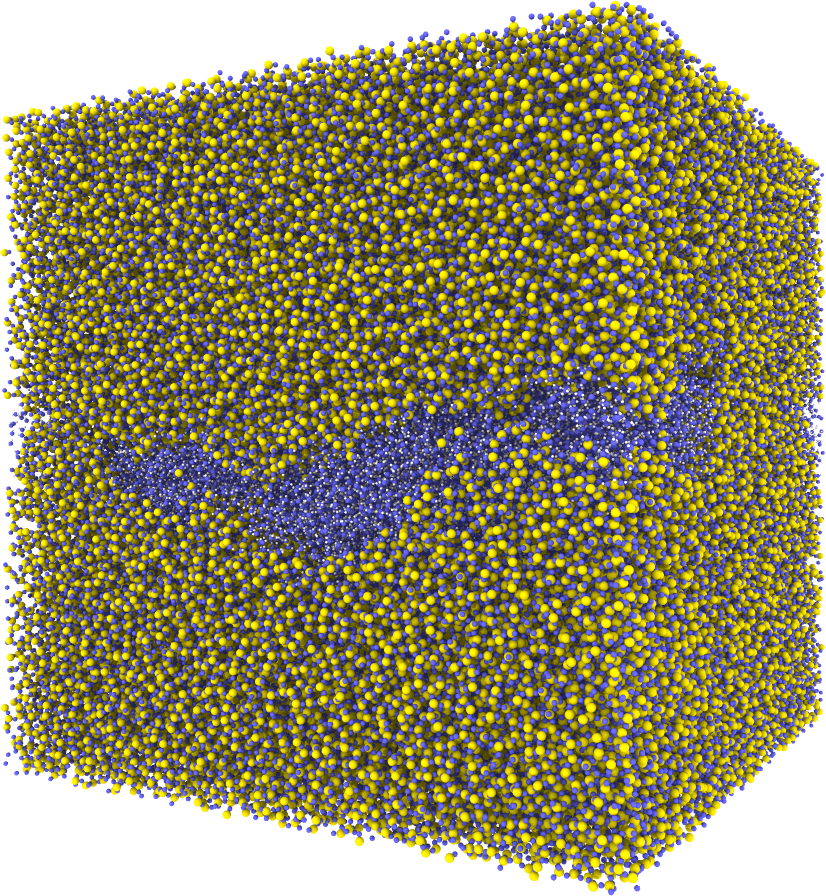
\includegraphics[width=\textwidth]{images/systems/trimmed-rough_fracture01_abel_13}%
            \caption{The whole system.}%
        \end{subfigure}%
        \hspace{\myhfillwidth}%
        \begin{subfigure}[t]{\myfigwidth}%
            \centering%
            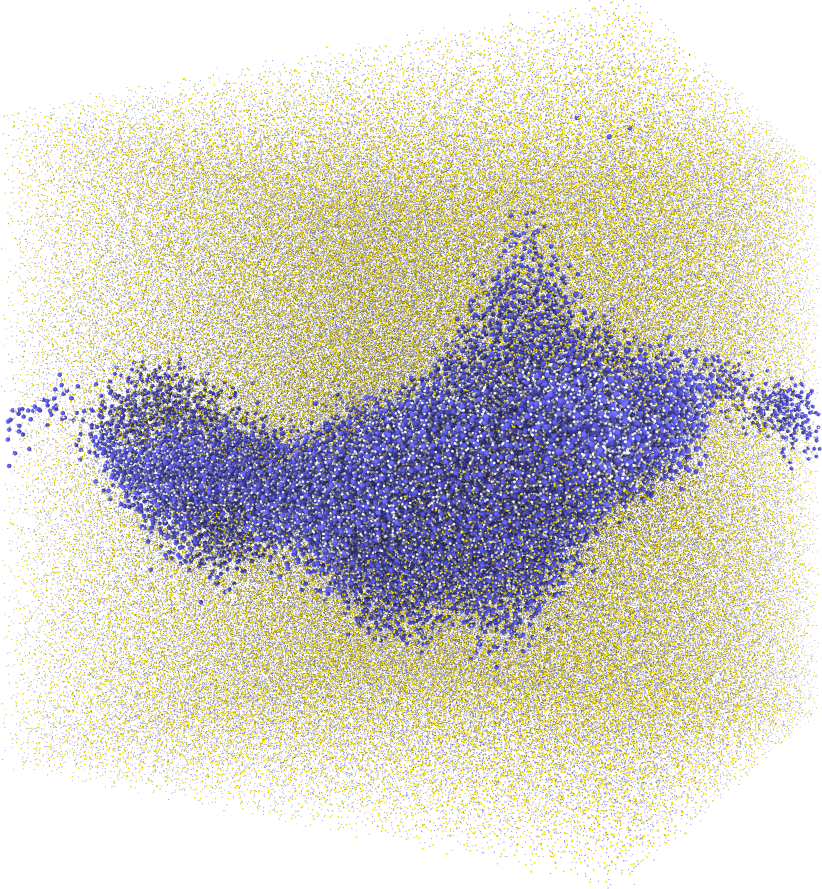
\includegraphics[width=\textwidth]{images/systems/trimmed-rough_fracture01_abel_15}%
            \caption{The whole system, with the size of the silicon and silica-oxygen atoms reduced to 0.1 \AA.}%
        \end{subfigure}%
    }%
        \vspace{10pt}\\%
    \makebox[\textwidth][c]{%
        \begin{subfigure}[t]{\myfigwidth}%
            \centering%
            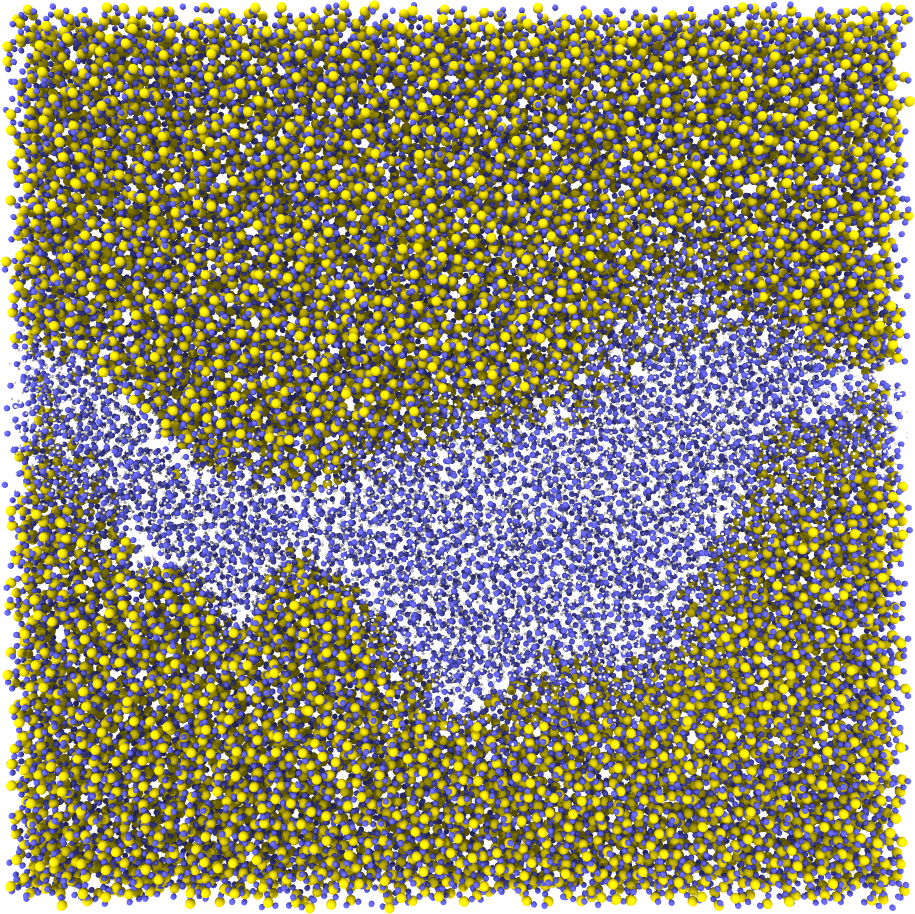
\includegraphics[width=\textwidth]{images/systems/trimmed-rough_fracture01_abel_16}%
            \caption{20 \AA\ thick slice.}%
        \end{subfigure}%
        \hspace{\myhfillwidth}%
        \begin{subfigure}[t]{\myfigwidth}%
            \centering%
            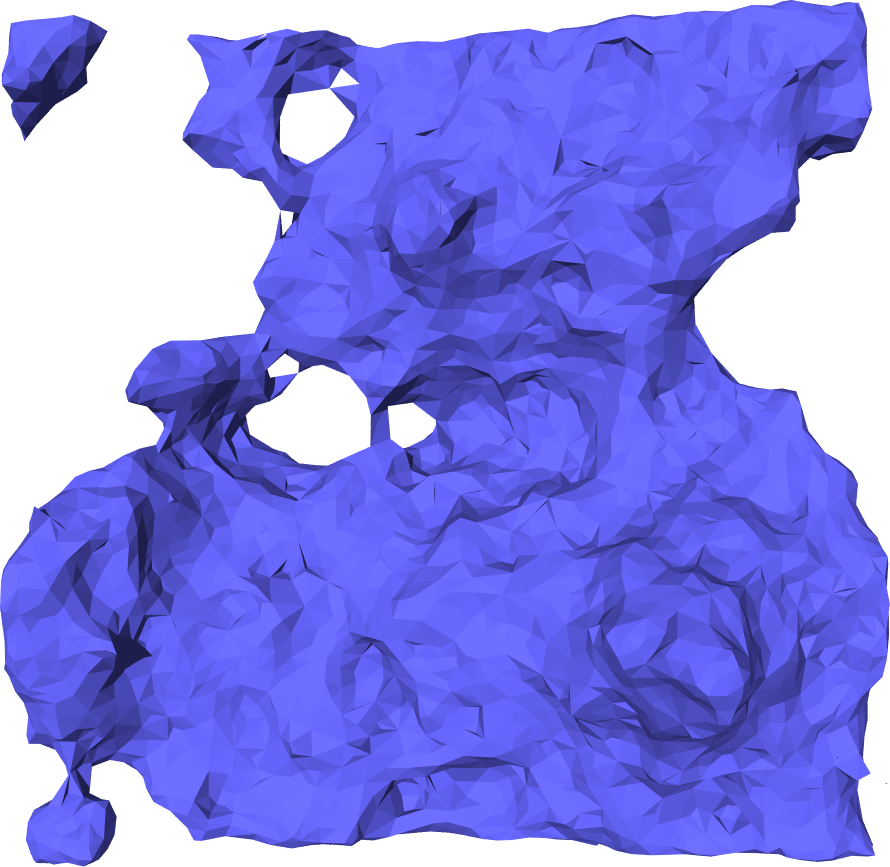
\includegraphics[width=\textwidth]{images/systems/trimmed-rough_fracture01_abel_22}%
            \caption{The pore volume.}%
        \end{subfigure}%
    }%
    \vspace{10pt}\\%
    \caption{%
        ``Rough fracture \#1'', a randomly generated fracture with varying width. Generated from two random surfaces. The size of this system is $179 \times 179 \times 179$.%
        \label{fig:renderings_rough_fracture01_abel}%
    }%
\end{figure}%


% ---- rough_fracture03 ---- %
%
\begin{figure}[!p]%
    \centering%
    \setlength{\myfigwidth}{0.55\textwidth}%
    \setlength{\myhfillwidth}{5mm}%
    %     \setlength{\mycaptionwidth}{0.3\textwidth}%
    %
    % Use makebox to center figures below that are wider than \textwidth
    % Use \centering inside subfigure to center image over caption
    %
    \makebox[\textwidth][c]{%
        \begin{subfigure}[t]{\myfigwidth}%
            \centering%
            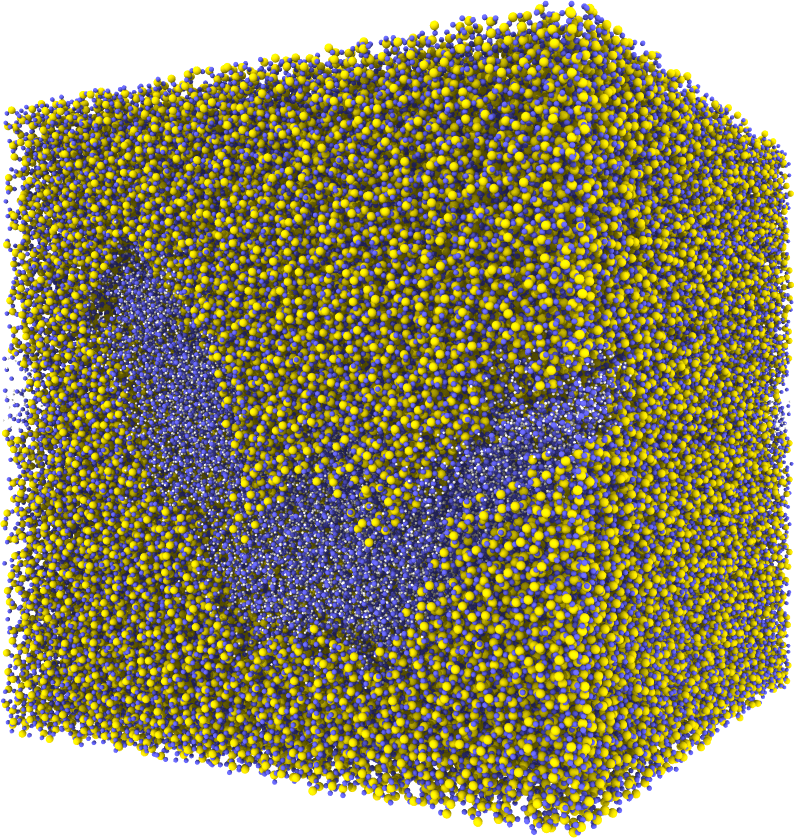
\includegraphics[width=\textwidth]{images/systems/trimmed-rough_fracture03_06}%
            \caption{The whole system.}%
        \end{subfigure}%
        \hspace{\myhfillwidth}%
        \begin{subfigure}[t]{\myfigwidth}%
            \centering%
            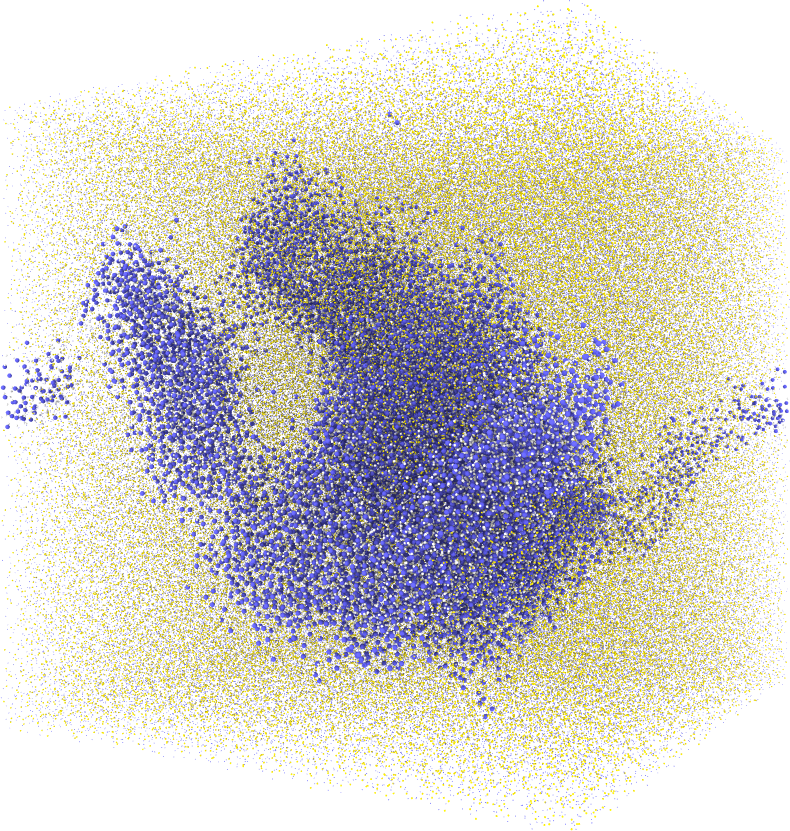
\includegraphics[width=\textwidth]{images/systems/trimmed-rough_fracture03_05}%
            \caption{The whole system, with the size of the silicon and silica-oxygen atoms reduced to 0.1 \AA.}%
        \end{subfigure}%
    }%
    \vspace{10pt}\\%
    \makebox[\textwidth][c]{%
        \begin{subfigure}[t]{\myfigwidth}%
            \centering%
            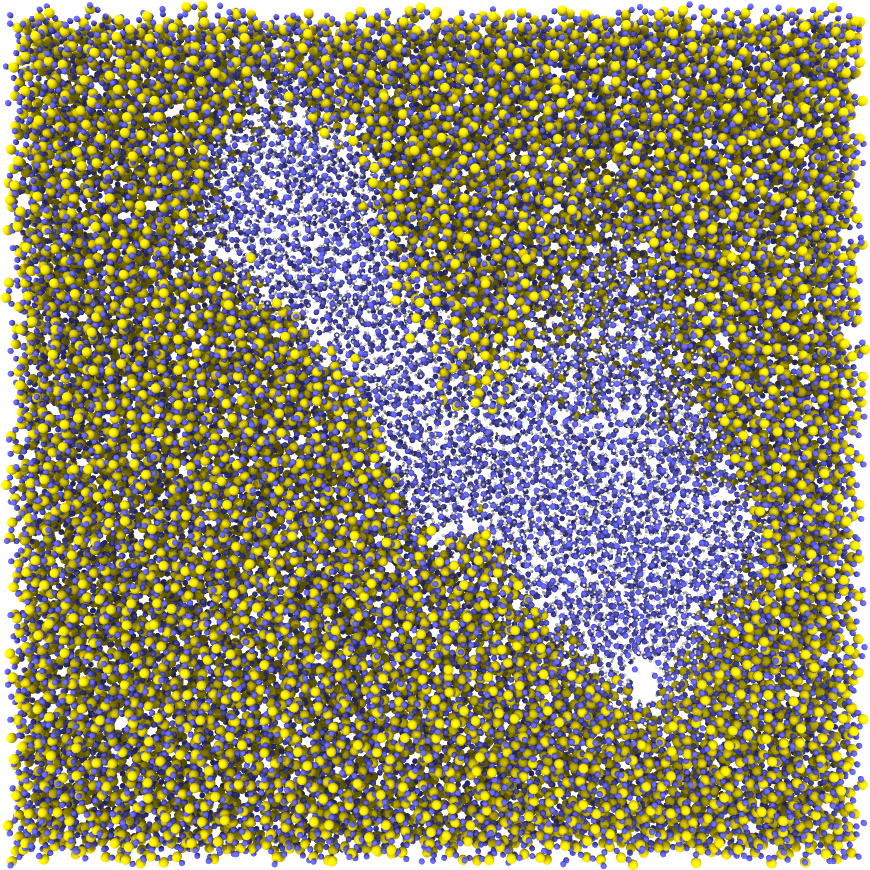
\includegraphics[width=\textwidth]{images/systems/trimmed-rough_fracture03_07}%
            \caption{20 \AA\ thick slice.}%
        \end{subfigure}%
        \hspace{\myhfillwidth}%
        \begin{subfigure}[t]{\myfigwidth}%
            \centering%
            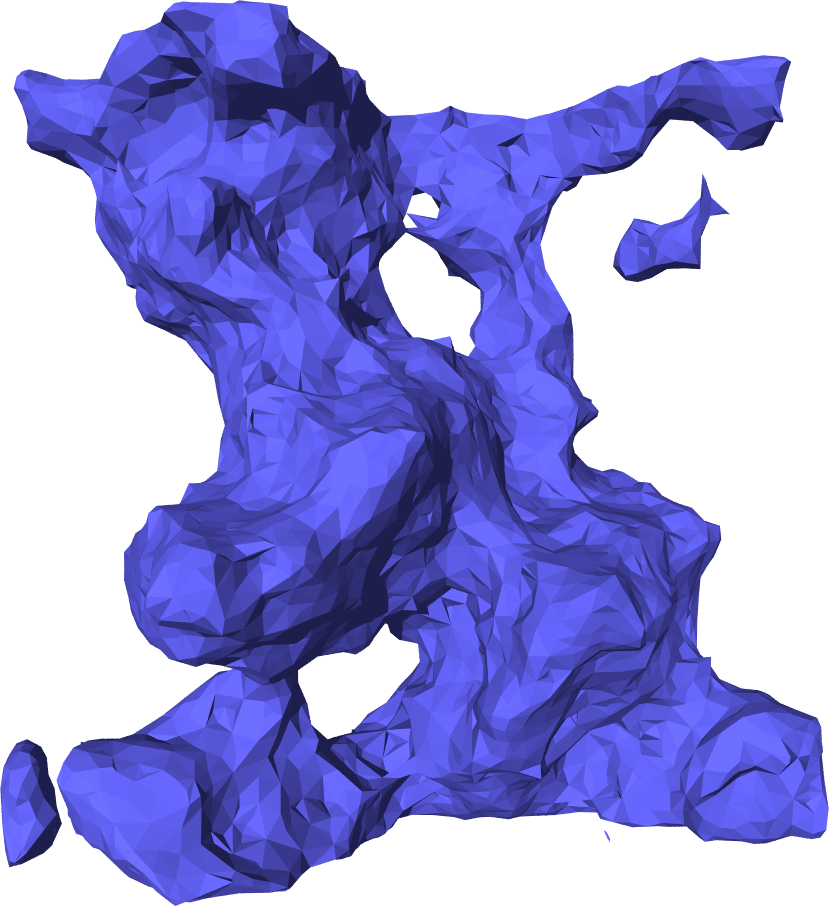
\includegraphics[width=\textwidth]{images/systems/trimmed-rough_fracture03_11}%
            \caption{The pore volume.}%
        \end{subfigure}%
    }%
    \vspace{10pt}\\%
    \caption{%
        ``Rough fracture \#2'', a randomly generated fracture with varying width. Generated from two random surfaces. The size of this system is $172 \times 172 \times 172$.%
        \label{fig:renderings_rough_fracture03}%
    }%
\end{figure}%


% ---- rough_fracture04_same_distance ---- %
%
\begin{figure}[!p]%
    \centering%
    \setlength{\myfigwidth}{0.55\textwidth}%
    \setlength{\myhfillwidth}{5mm}%
    %     \setlength{\mycaptionwidth}{0.3\textwidth}%
    %
    % Use makebox to center figures below that are wider than \textwidth
    % Use \centering inside subfigure to center image over caption
    %
    \makebox[\textwidth][c]{%
        \begin{subfigure}[t]{\myfigwidth}%
            \centering%
            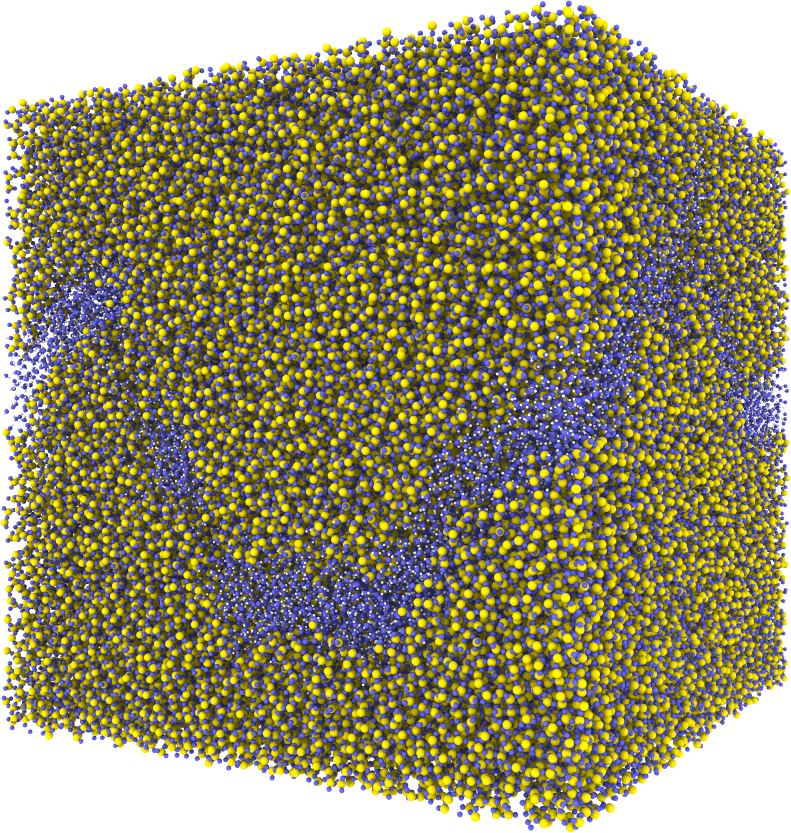
\includegraphics[width=\textwidth]{images/systems/trimmed-rough_fracture04_06}%
            \caption{The whole system.}%
        \end{subfigure}%
        \hspace{\myhfillwidth}%
        \begin{subfigure}[t]{\myfigwidth}%
            \centering%
            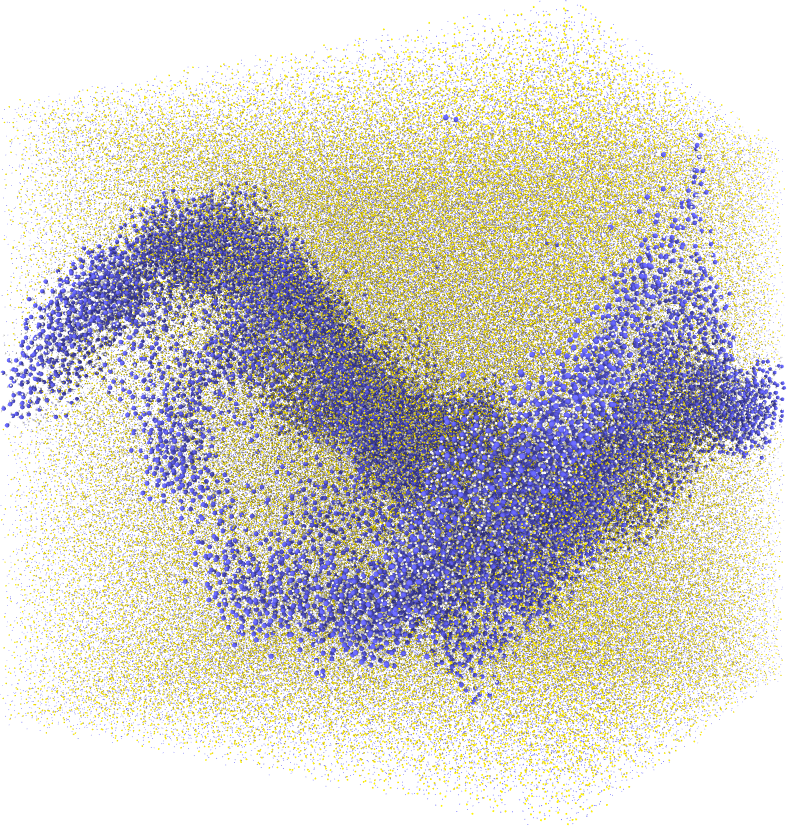
\includegraphics[width=\textwidth]{images/systems/trimmed-rough_fracture04_07}%
            \caption{The whole system, with the size of the silicon and silica-oxygen atoms reduced to 0.1 \AA.}%
        \end{subfigure}%
    }%
    \vspace{10pt}\\%
    \makebox[\textwidth][c]{%
        \begin{subfigure}[t]{\myfigwidth}%
            \centering%
            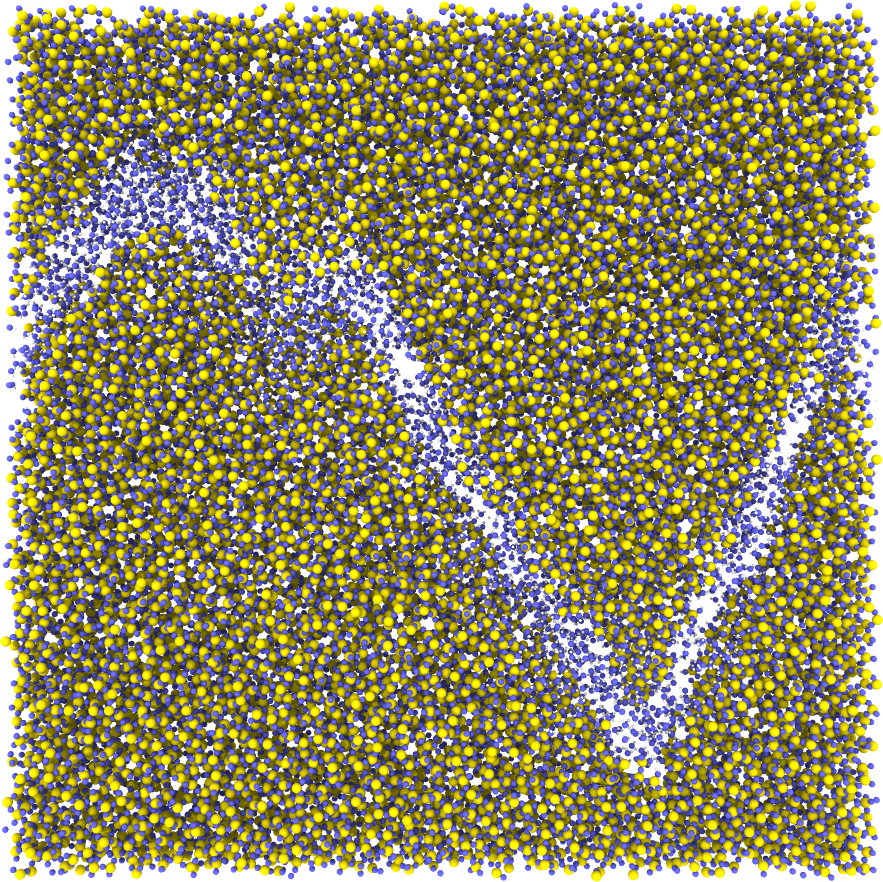
\includegraphics[width=\textwidth]{images/systems/trimmed-rough_fracture04_05_20ang}%
            \caption{20 \AA\ thick slice.}%
        \end{subfigure}%
        \hspace{\myhfillwidth}%
        \begin{subfigure}[t]{\myfigwidth}%
            \centering%
            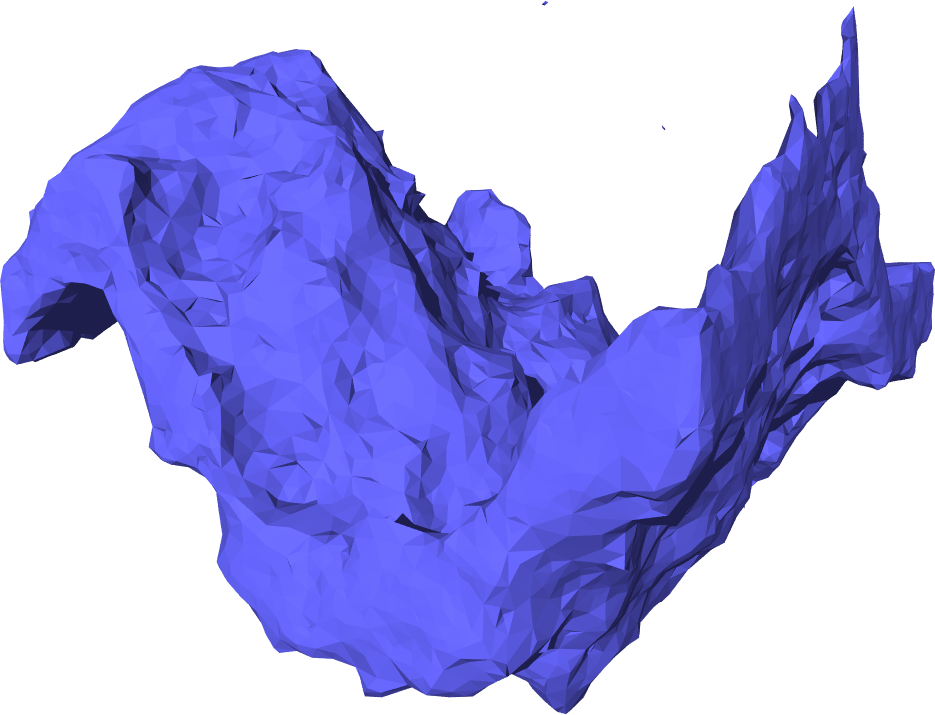
\includegraphics[width=\textwidth]{images/systems/trimmed-rough_fracture04_11}%
            \caption{The pore volume.}%
        \end{subfigure}%
    }%
    \vspace{10pt}\\%
    \caption{%
        ``Rough fracture \#3'', a randomly generated fracture generated from one surface repeated for the top and bottom half, with 14.4 \AA\ between the surfaces, giving approximately uniform width of the pore. The size of this system is $172 \times 172 \times 172$.%
        \label{fig:renderings_rough_fracture04_same_distance}%
    }%
\end{figure}%


% ---- rough_fracture05 ---- %
\begin{figure}[!p]%
    \centering%
    \setlength{\myfigwidth}{0.55\textwidth}%
    \setlength{\myhfillwidth}{5mm}%
    %     \setlength{\mycaptionwidth}{0.3\textwidth}%
    %
    % Use makebox to center figures below that are wider than \textwidth
    % Use \centering inside subfigure to center image over caption
    %
    \makebox[\textwidth][c]{%
        \begin{subfigure}[t]{\myfigwidth}%
            \centering%
            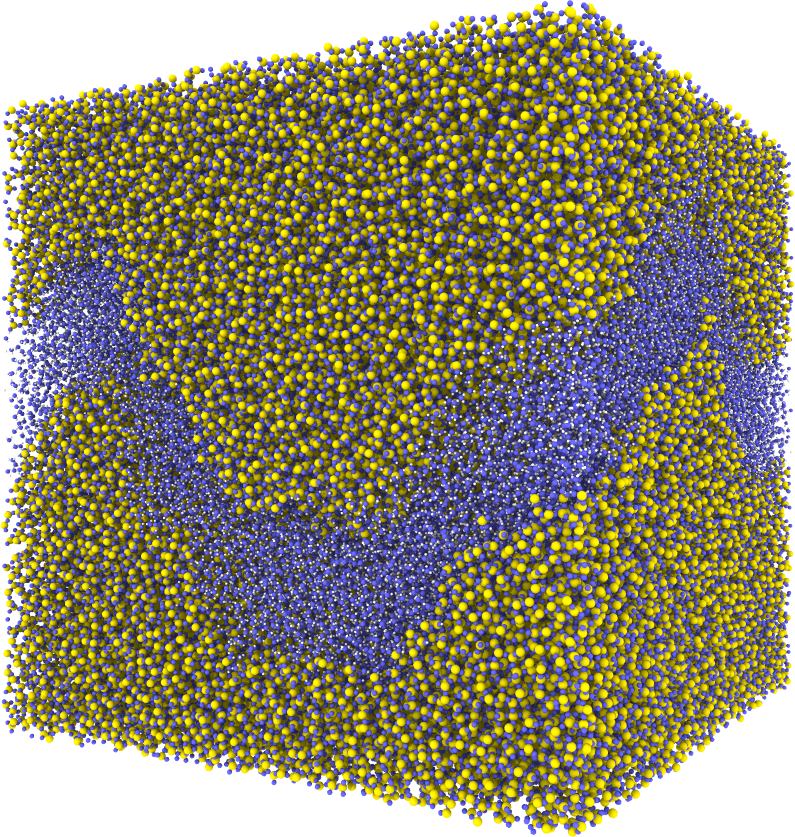
\includegraphics[width=\textwidth]{images/systems/trimmed-rough_fracture05_05}%
            \caption{The whole system.}%
        \end{subfigure}%
        \hspace{\myhfillwidth}%
        \begin{subfigure}[t]{\myfigwidth}%
            \centering%
            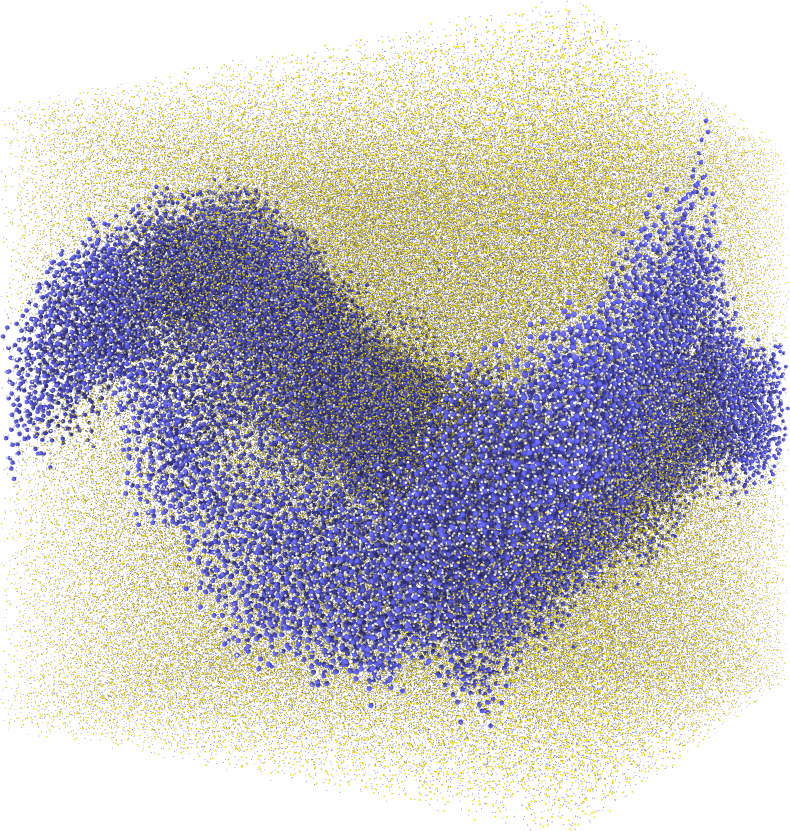
\includegraphics[width=\textwidth]{images/systems/trimmed-rough_fracture05_04}%
            \caption{The whole system, with the size of the silicon and silica-oxygen atoms reduced to 0.1 \AA.}%
        \end{subfigure}%
    }%
    \vspace{10pt}\\%
    \makebox[\textwidth][c]{%
        \begin{subfigure}[t]{\myfigwidth}%
            \centering%
            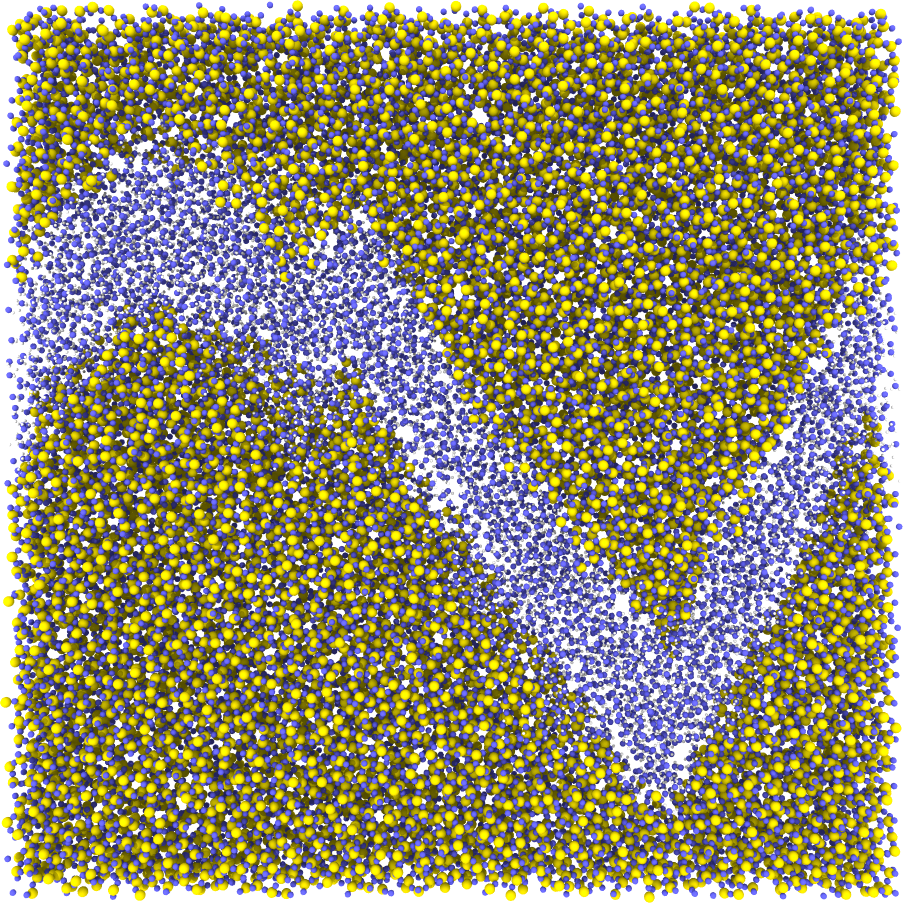
\includegraphics[width=\textwidth]{images/systems/trimmed-rough_fracture05_02_20ang}%
            \caption{20 \AA\ thick slice.}%
        \end{subfigure}%
        \hspace{\myhfillwidth}%
        \begin{subfigure}[t]{\myfigwidth}%
            \centering%
            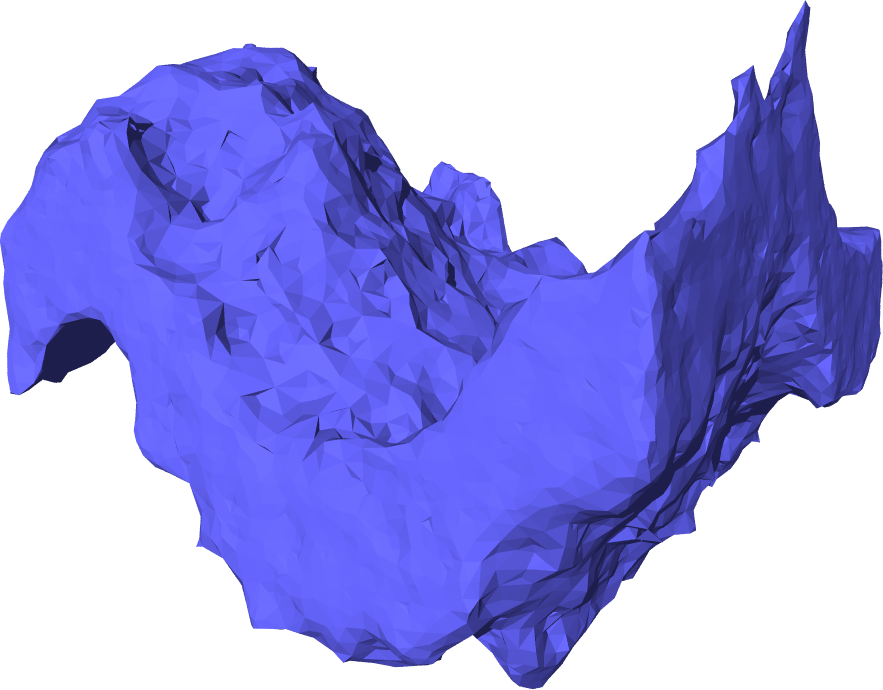
\includegraphics[width=\textwidth]{images/systems/trimmed-rough_fracture05_09}%
            \caption{The pore volume.}%
        \end{subfigure}%
    }%
    \vspace{10pt}\\%
    \caption{%
        ``Rough fracture \#4'', a randomly generated fracture generated from one surface repeated for the top and bottom half, with 28.8 \AA\ between the surfaces, giving approximately uniform width of the pore.  The size of this system is $172 \times 172 \times 172$. %
        \label{fig:renderings_rough_fracture05}%
    }%
\end{figure}%


% ---- Reference systems ---- %
%
\begin{figure}[htpb]%
%     \centering%
    \setlength{\myfigwidth}{0.55\textwidth}%
    \setlength{\myhfillwidth}{5mm}%
    %     \setlength{\mycaptionwidth}{0.3\textwidth}%
    %
    % Use makebox to center figures below that are wider than \textwidth
    % Use \centering inside subfigure to center image over caption
    %
    \makebox[\textwidth][c]{%
        \begin{subfigure}[t]{\myfigwidth}%
            \centering%
            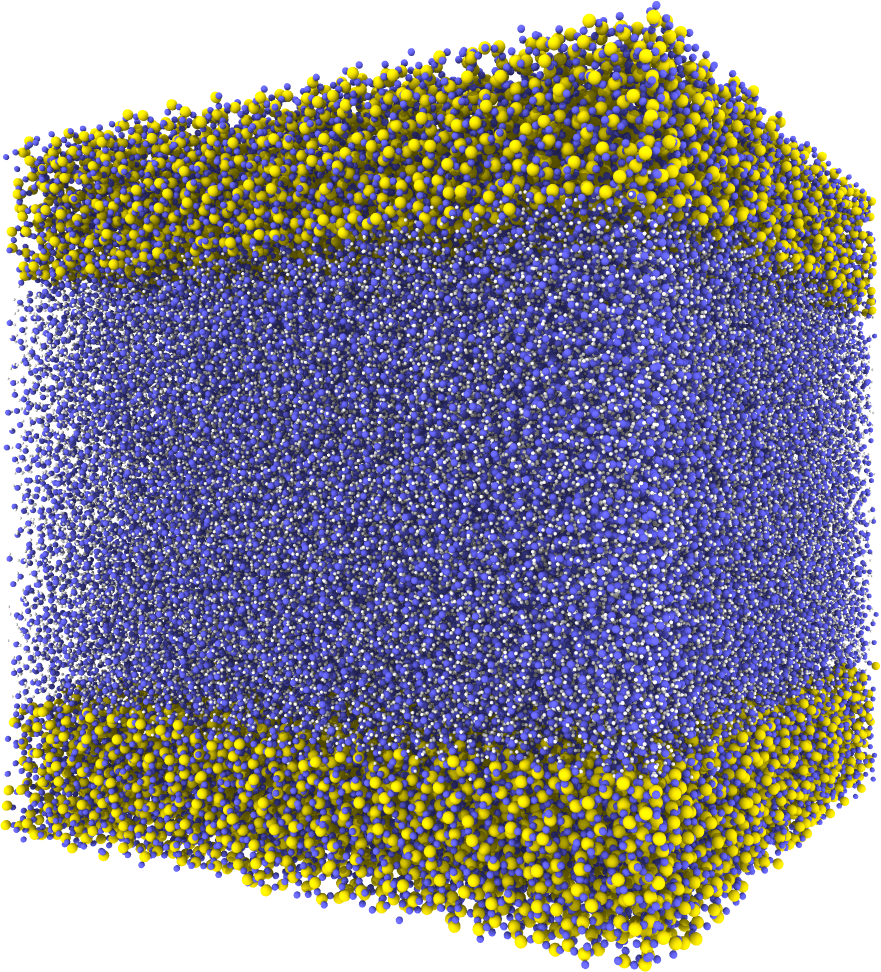
\includegraphics[width=\textwidth]{images/systems/trimmed-flat_square_fracture02_03}%
            \caption{``Reference \#1''.}%
            \label{fig:renderings_flat_square_fracture02}%
        \end{subfigure}%
        \hspace{\myhfillwidth}%
        \begin{subfigure}[t]{\myfigwidth}%
            \centering%
            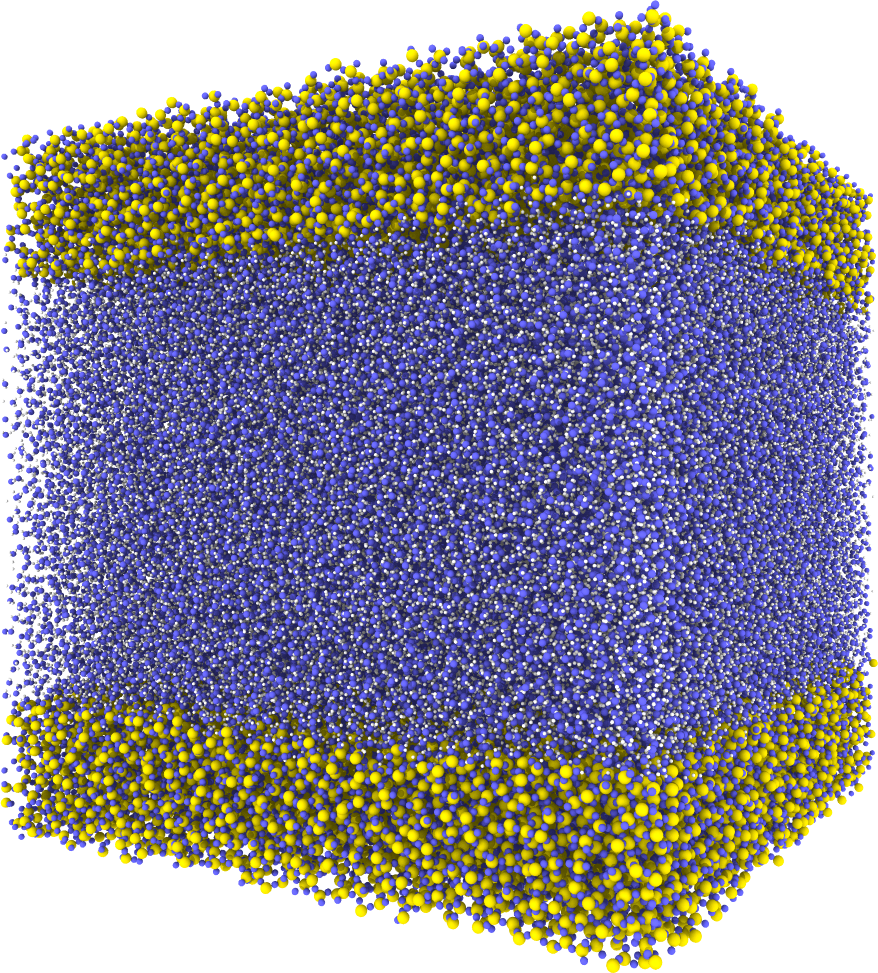
\includegraphics[width=\textwidth]{images/systems/trimmed-flat_square_fracture03_04}%
            \caption{``Reference \#2''.}%
            \label{fig:renderings_flat_square_fracture03}%
        \end{subfigure}%
    }%
    \vspace{10pt}\\%
    \caption{%
        Reference systems \#1 and \#2, 86 \AA\ wide flat pores. Both these systems have size $179 \times 179 \times 179$.%
        \label{fig:renderings_flat_fractures01}%
    }%
\end{figure}%


% ---- Reference systems ---- %
%
\begin{figure}[htpb]%
%     \centering%
    \setlength{\myfigwidth}{0.55\textwidth}%
    \setlength{\myhfillwidth}{5mm}%
    %     \setlength{\mycaptionwidth}{0.3\textwidth}%
    %
    % Use makebox to center figures below that are wider than \textwidth
    % Use \centering inside subfigure to center image over caption
    %
    \makebox[\textwidth][c]{%
        \begin{subfigure}[t]{\myfigwidth}%
            \centering%
            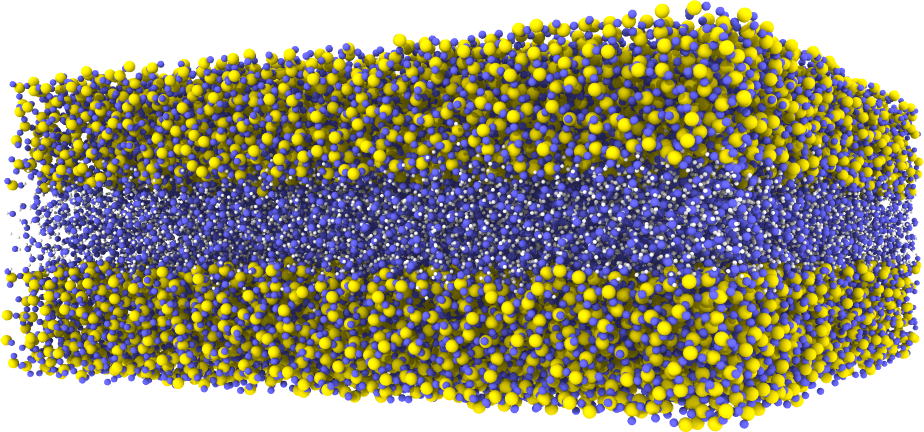
\includegraphics[width=\textwidth]{images/systems/trimmed-flat_fracture02_03}%
            \caption{``Reference \#3''.}%
            \label{fig:renderings_flat_fracture02}%
        \end{subfigure}%
        \hspace{\myhfillwidth}%
        \begin{subfigure}[t]{\myfigwidth}%
            \centering%
            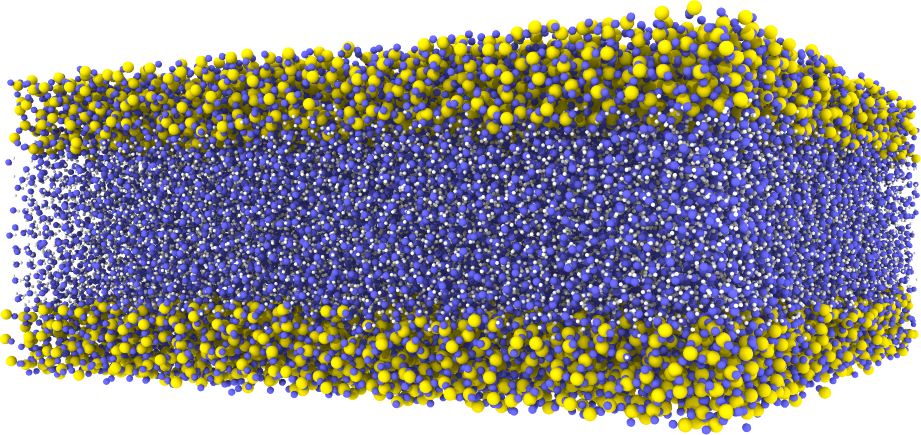
\includegraphics[width=\textwidth]{images/systems/trimmed-flat_fracture03_03}%
            \caption{``Reference \#4''.}%
            \label{fig:renderings_flat_fracture03}%
        \end{subfigure}%
    }%
    \vspace{10pt}\\%
    \caption{%
        Reference systems \#3 and \#4, respective a 14.4 and a 28.8 \AA\ wide flat pore. Both these systems have size $143 \times 143 \times 57$.%
        \label{fig:renderings_flat_fractures02}%
    }%
\end{figure}%